\section{AlexNet}\label{sec:alexnet}
In this section I will describe the AlexNet architecture and the results obtained using it.

\subsection{Architecture}\label{sec:alexnet-architecture}
The AlexNet architecture is a convolutional neural network designed by Alex Krizhevsky, Ilya Sutskever and Geoffrey Hinton in 2012.
It was the first architecture that won the ImageNet Large Scale Visual Recognition Challenge (ILSVRC) in 2012.
The architecture is structured as follows:
\begin{itemize}
    \item \textbf{Input}: 256$\times$256$\times$3
    \item \textbf{Convolution}: 96 filters of size 11$\times$11$\times$3 with stride 4 and padding valid
    \item \textbf{Max Pooling}: 3$\times$3 with stride 2
    \item \textbf{Convolution}: 256 filters of size 5$\times$5$\times$96 with stride 1 and padding same
    \item \textbf{Max Pooling}: 3$\times$3 with stride 2
    \item \textbf{Convolution}: 384 filters of size 3$\times$3$\times$256 with stride 1 and padding same
    \item \textbf{Convolution}: 384 filters of size 3$\times$3$\times$384 with stride 1 and padding same
    \item \textbf{Convolution}: 256 filters of size 3$\times$3$\times$384 with stride 1 and padding same
    \item \textbf{Max Pooling}: 3$\times$3 with stride 2
    \item \textbf{Flatten}
    \item \textbf{Dense}: 4096 neurons
    \item \textbf{Dropout}: rate 0.5
    \item \textbf{Dense}: 4096 neurons
    \item \textbf{Dropout}: rate 0.5
    \item \textbf{Dense}: 10 neurons
\end{itemize}
\newpage
\subsection{Training}\label{sec:alexnet-training}
I have trained two AlexNet models with different learning rates (0.001 and 0.0001) using the Adam optimizer.
It has been trained using Google Colab with a GPU runtime and the training took about 1 hour for each model.
The training and validation accuracy and loss are shown in Figure~\ref{fig:alexnet-accuracy} and Figure~\ref{fig:alexnet-loss}.
As we can see, a learning rate of 0.001 is too high and the model does not converge.

\begin{figure}[h]
    \centering
    \subfloat[\centering Learning Rate = 0.001]{{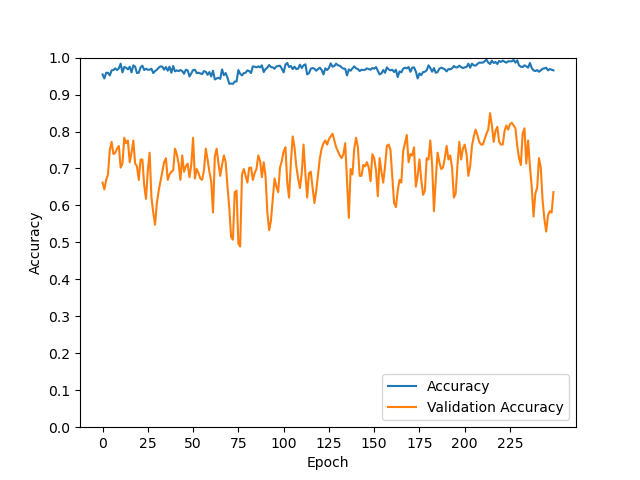
\includegraphics[width=0.45\textwidth]{../plot/lr-0001/alexnet-accuracy.png}}}
    \qquad
    \subfloat[\centering Learning Rate = 0.0001]{{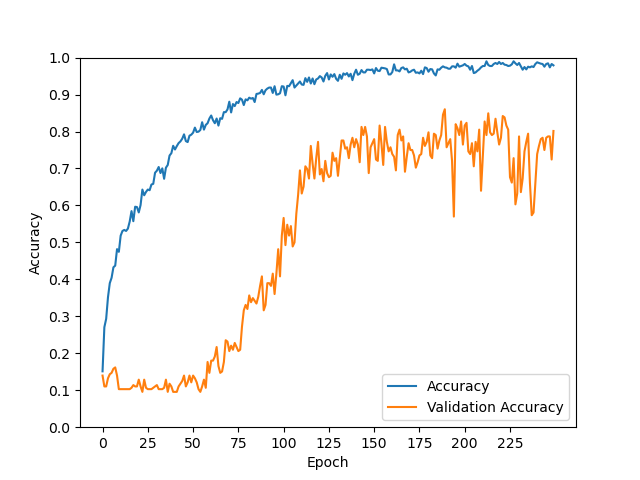
\includegraphics[width=0.45\textwidth]{../plot/lr-00001/alexnet-accuracy.png}}}
    \caption{Training and validation accuracy for the AlexNet with different learning rates}\label{fig:alexnet-accuracy}
\end{figure}

\begin{figure}[h]
    \centering
    \subfloat[\centering Learning Rate = 0.001]{{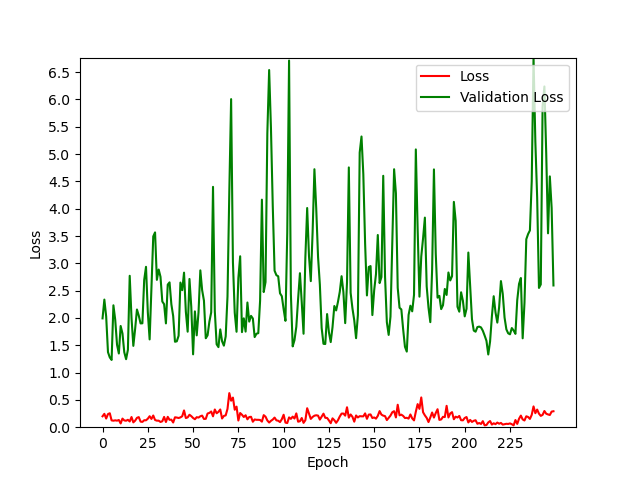
\includegraphics[width=0.45\textwidth]{../plot/lr-0001/alexnet-loss.png}}}
    \qquad
    \subfloat[\centering Learning Rate = 0.0001]{{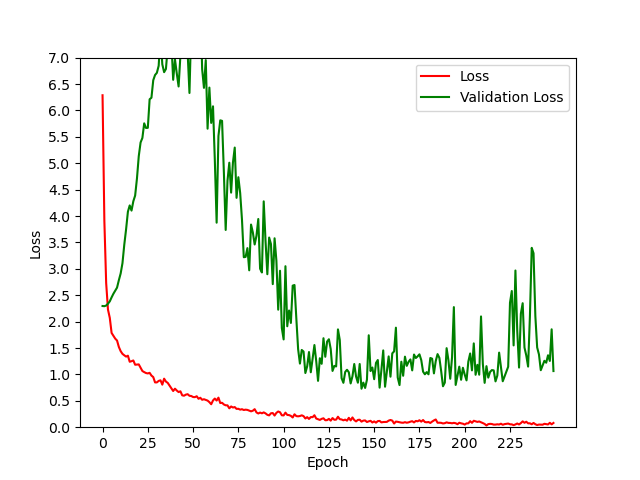
\includegraphics[width=0.45\textwidth]{../plot/lr-00001/alexnet-loss.png}}}
    \caption{Training and validation loss for the AlexNet with different learning rates}\label{fig:alexnet-loss}
\end{figure}

\subsection{Evaluation}\label{sec:alexnet-evaluation}
The model was evaluated using the test dataset and the results are shown in the confusion matrix in Figure~\ref{fig:alexnet-confusion-matrix}.
The accuracy, precision, recall, F1-score and AUC are shown in Table~\ref{tab:results-alexnet}.

As we can see from the results, the model model with a learning rate of 0.0001 performs better than the one with a learning rate of 0.001.
However, the model with a learning rate of 0.0001 still has a low accuracy and the AUC is not very high.
Looking at the confusion matrix, we can see that the model is not able to distinguish between the classes 0 and 9 which are the most similar.

\begin{figure}[h]
    \centering
    \subfloat[\centering Learning Rate = 0.001]{{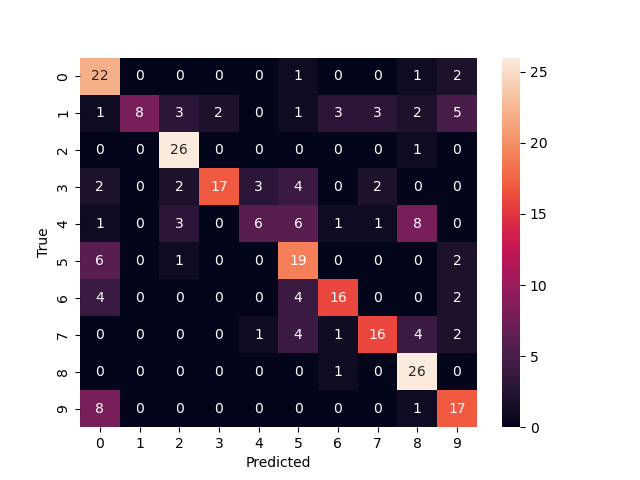
\includegraphics[width=0.45\textwidth]{../plot/lr-0001/alexnet-confusion-matrix.png}}}
    \qquad
    \subfloat[\centering Learning Rate = 0.0001]{{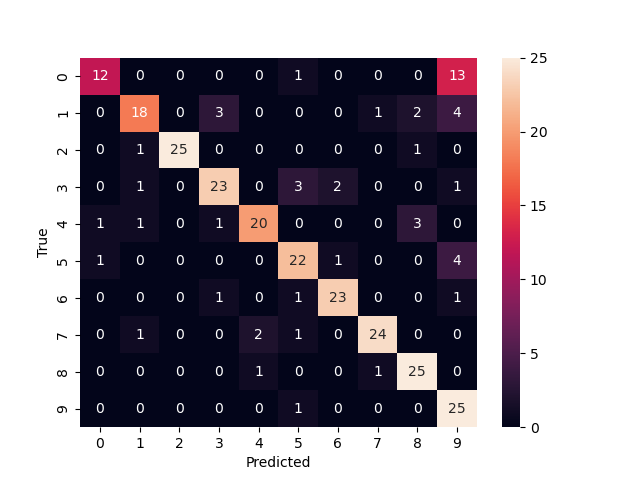
\includegraphics[width=0.45\textwidth]{../plot/lr-00001/alexnet-confusion-matrix.png}}}
    \caption{Confusion matrix for the AlexNet with different learning rates}\label{fig:alexnet-confusion-matrix}
\end{figure}

\begin{table}[h]
    \centering
    \begin{tabular}{|c|c|c|c|c|c|}
        \hline
        \textbf{LR}     & \textbf{Accuracy} & \textbf{Precision} & \textbf{Recall} & \textbf{F1-Score} & \textbf{AUC} \\
        \hline
        \textbf{0.001}  & 0.6985            & 0.9748             & 0.9431          & 0.9587            & 0.8562       \\
        \hline
        \textbf{0.0001} & 0.7977            & 0.9457             & 0.9919          & 0.9683            & 0.7267       \\
        \hline
    \end{tabular}
    \caption{Evaluation of the AlexNet with different learning rates}\label{tab:results-alexnet}
\end{table}